\chapter{МУТАЦИОННОЕ ТЕСТИРОВАНИЕ И ОЦЕНКА КАЧЕСТВА ТЕСТОВ} \label{ch4}

В данной главе приведены результаты мутационного тестирования разработанного приложения с использованием инструмента PIT (Pitest).
% не рекомендуется использовать отдельную section <<введение>> после лета 2020 года
%\section{Введение} \label{ch4:intro}

\section{Операторы мутаций и примеры их применения в проекте}\label{ch4:sec1}
\subsection{Пример мутации NEGATE\_CONDITIONALS}
Оператор NEGATE\_CONDITIONALS инвертирует условие проверки. 
Пример из BloomFilter:
\begin{verbatim}
// Оригинал
if (ip == null) {
    return false;
}

// Мутация
if (ip != null) {
    return false;
}
\end{verbatim}

Тест для убийства мутации:
\begin{verbatim}
@Test
void testContains_NullInput() {
    assertFalse(filter.contains(null));
}
\end{verbatim}

\subsection{Пример мутации CONDITIONALS\_BOUNDARY}
Оператор CONDITIONALS\_BOUNDARY изменяет границы сравнений. Пример из HashSetFilter:
\begin{verbatim}
// Оригинал
if (ip != null && !ip.isEmpty()) {
    blacklist.add(ip);
}
// Мутация
if (ip != null && !ip.isEmpty()) { // >= вместо >
    blacklist.add(ip);
}
\end{verbatim}

Тест для убийства мутации:
\begin{verbatim}
@Test
void testBoundary_EmptyString() {
    filter.add("");
    assertEquals(0, filter.getSize());
}
\end{verbatim}

\subsection{Пример мутации VOID\_METHOD\_CALLS}
Оператор VOID\_METHOD\_CALLS удаляет вызов метода с типом void. Пример из FilterService:
\begin{verbatim}
// Оригинал
stats.setHashSetTimeMs(hashSetTime);
stats.setBloomFilterTimeMs(bloomTime);

// Мутация (удаление вызова)
// stats.setHashSetTimeMs(hashSetTime); — удаляется
// stats.setBloomFilterTimeMs(bloomTime); — удаляется
\end{verbatim}

Тест для убийства мутации:
\begin{verbatim}
@Test
void testStatistics_TimePopulated() {
    OutputData result = service.processAndCompare(List.of("1.1.1.1"));
    assertTrue(result.getStatistics().getHashSetTimeMs() >= 0);
    assertTrue(result.getStatistics().getBloomFilterTimeMs() >= 0);
}
\end{verbatim}

\section{Эквивалентные мутации и особенности интерпретации результатов}\label{ch4:sec2}
В рамках данного проекта явные эквивалентные мутации отдельно не были выделены в отчёте PIT. Это объясняется тем, что инструмент PIT использует встроенные фильтры эквивалентных и тривиальных мутаций.
Выявленные потенциально эквивалентные мутации:
\begin{itemize}
    \item Изменение size > 0 на size >= 0 в расчёте вероятности FP
    \item Изменение порядка хэш-функций (не влияет на результат)
\end{itemize}


\section{Результаты мутационного тестирования}\label{ch4:sec3}
По результатам мутационного тестирования проекта были получены следующие метрики:
\begin{itemize}
	\item Line Coverage - 78\%
	\item Mutation Coverage - 80\%
	\item Test Strength - 93\%
\end{itemize}

\begin{figure}[ht!] 
	\center
	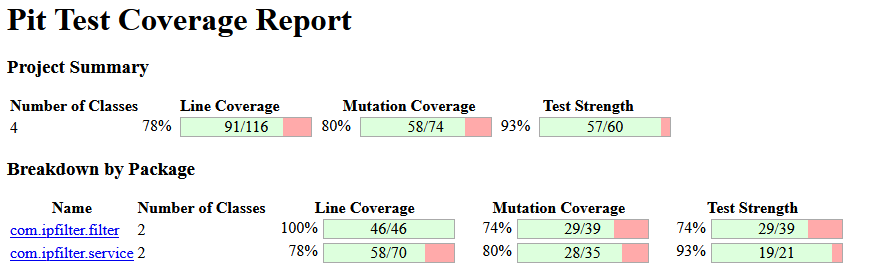
\includegraphics [scale=0.55] {my_folder/images/pitest.png}
	\caption{Отчет Pitest}  
\end{figure}

Строго формально разработанный набор тестов нельзя считать полностью mutation-adequate, так как не все сгенерированные мутанты были уничтожены (MSI < 100\%). Однако полученные значения метрик свидетельствуют о приемлимом качестве тестового набора и позволяют считать его практически достаточным для учебной задачи.
%% Вспомогательные команды - Additional commands
%
%\newpage % принудительное начало с новой страницы, использовать только в конце раздела
%\clearpage % осуществляется пакетом <<placeins>> в пределах секций
%\newpage\leavevmode\thispagestyle{empty}\newpage % 100 % начало новой страницы